\section{Application : Remplissage d'un ellipse}
\begin{enumerate}[(a)]
  \item On considère l'ellipse définit par le point $\overrightarrow{OM}(t) =
          (x(t), y(t)\in\mathbb{R}^2)$ où
        $
          \left\{
          \begin{array}{rcl}
            x' & = & 2x-5y \\
            y' & = & x-2y  \\
          \end{array}
          \right.
        $ avec les conditions initiales $M(0) = (1,2)$.\\
        \q{Tracer la courbe des points
          $M(t)$ pour $t\in [0, 2\pi]$ avec la méthode d'Euler en utilisant }
        \il{N = 80}\q{ points.}

        C'est là que je crée la classe \il{Ellipse} :
        \codeFromFileT{ressources/ellipse.py}{section-05/qa-1.py}
        \codeFromFileT{ressources/ellipse.py}{section-05/qa-2.py}
        Et je teste tout ça :
        \codeFromFileT{main.py}{section-05/qa-3.py}
        Pour obtenir :
        \begin{center}
          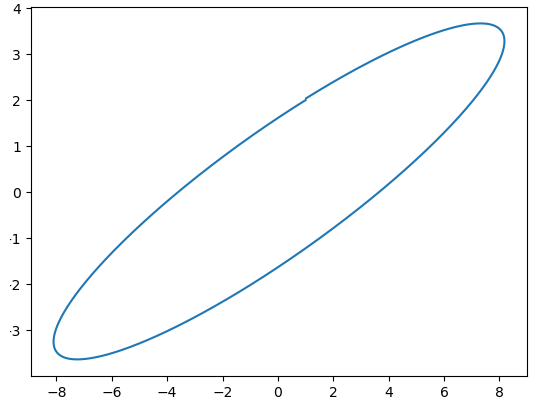
\includegraphics[scale=0.5]{section-05/qa-4.png}
        \end{center}
  \item \q{Trier tous les points de la courbe par abscisse croissante de manière
          à obtenir un quadrillage vertical de la courbe.}
        Aux vues des questions suivantes, je fais tous les remplissages d'un
        coup :
        \codeFromFileT{ressources/ellipse.py}{section-05/qb-1.py}
        Du coup je crée la mathode \il{separate} de la classe \il{Liste} :
        \codeFromFileT{ressources/liste.py}{section-05/qb-2.py}
        Je trace tout ça :
        \codeFromFileT{main.py}{section-05/qb-3.py}
        Et j'obtiens :
        \begin{center}
          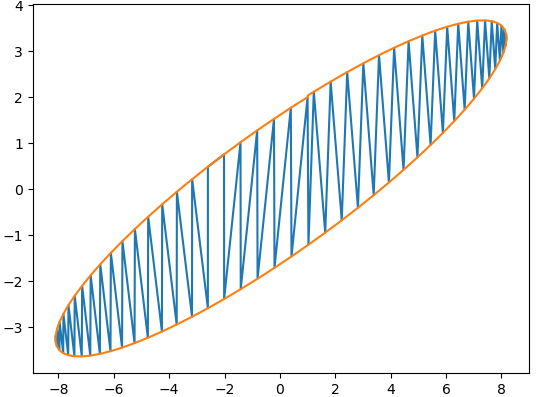
\includegraphics[scale=0.2]{section-05/qb-4.png}
        \end{center}
        
    \item \q{Trier tous les points de la courbe par ordonnée croissante de 
          manière à obtenir un quadrillage horizontal de la courbe.}
          \codeFromFileT{main.py}{section-05/qc-1.py}
          \begin{center}
            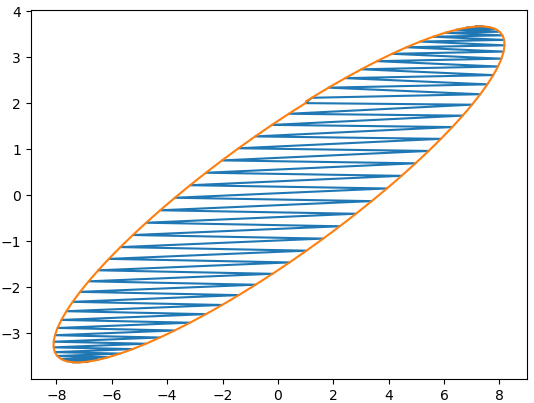
\includegraphics[scale=0.2]{section-05/qc-2.png}
          \end{center}
    \item \q{Trier tous les points de la courbe de 
          manière à obtenir un quadrillage radial de la courbe.}
          \codeFromFileT{main.py}{section-05/qd-1.py}
          \begin{center}
            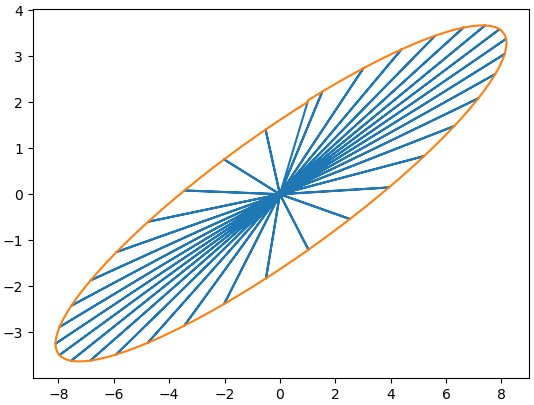
\includegraphics[scale=0.2]{section-05/qd-2.png}
          \end{center}



\end{enumerate}

